% Created by tikzDevice version 0.6.1 on 2011-06-27 00:25:12
% !TEX encoding = UTF-8 Unicode
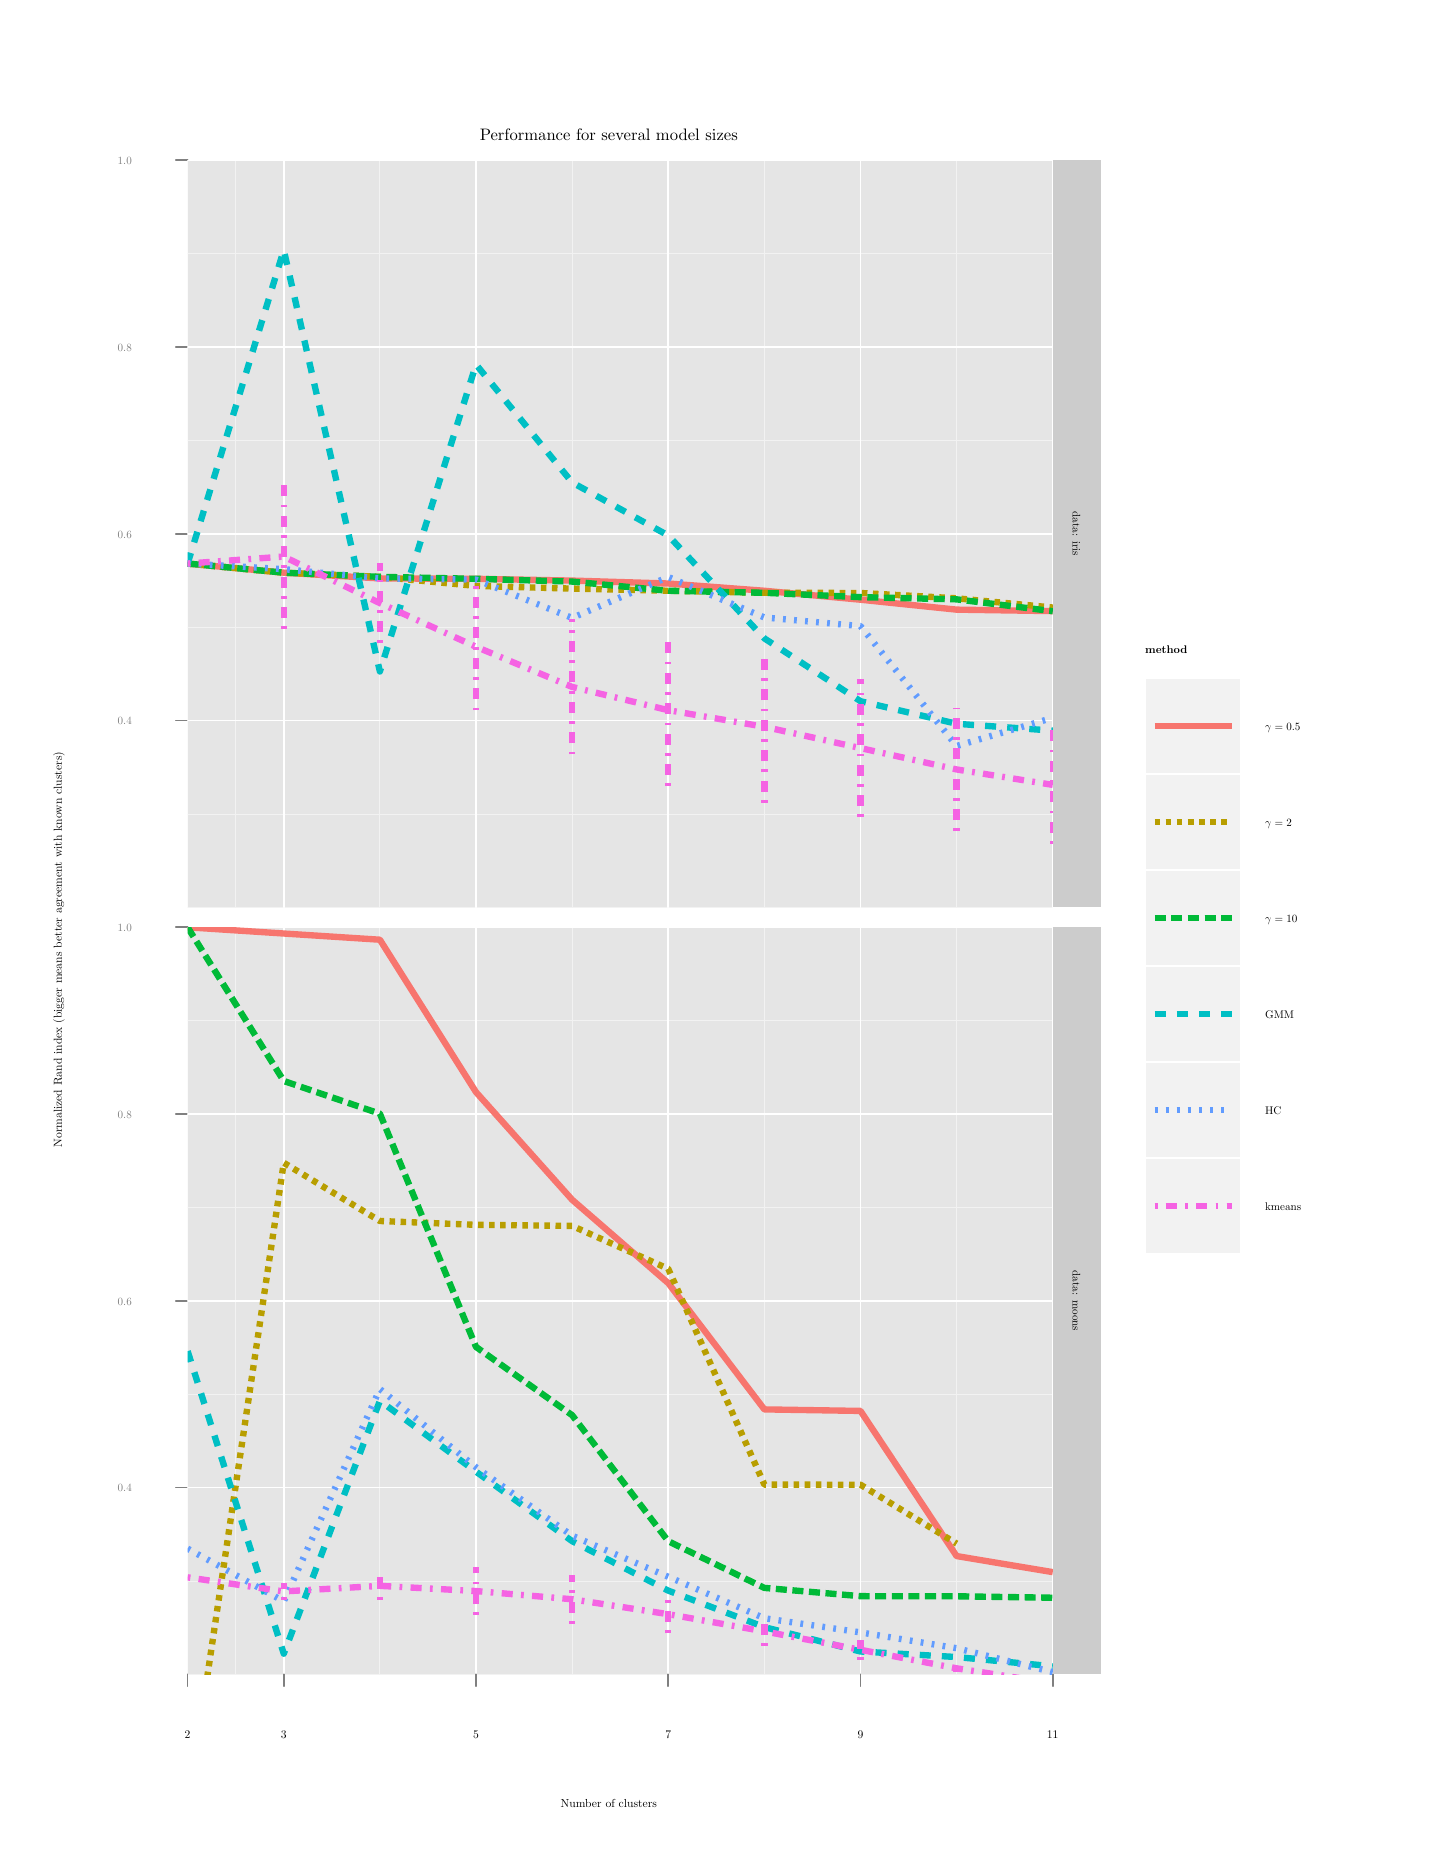
\begin{tikzpicture}[x=1pt,y=1pt]
\definecolor[named]{drawColor}{rgb}{0.00,0.00,0.00}
\definecolor[named]{fillColor}{rgb}{1.00,1.00,1.00}
\fill[color=fillColor,] (0,0) rectangle (505.89,650.43);
\begin{scope}
\path[clip] (  0.00,  0.00) rectangle (505.89,650.43);
\end{scope}
\begin{scope}
\path[clip] (  0.00,  0.00) rectangle (505.89,650.43);
\end{scope}
\begin{scope}
\path[clip] (  0.00,  0.00) rectangle (505.89,650.43);
\end{scope}
\begin{scope}
\path[clip] (  0.00,  0.00) rectangle (505.89,650.43);
\end{scope}
\begin{scope}
\path[clip] (  0.00,  0.00) rectangle (505.89,650.43);
\end{scope}
\begin{scope}
\path[clip] (  0.00,  0.00) rectangle (505.89,650.43);
\end{scope}
\begin{scope}
\path[clip] (  0.00,  0.00) rectangle (505.89,650.43);
\end{scope}
\begin{scope}
\path[clip] (  0.00,  0.00) rectangle (505.89,650.43);
\end{scope}
\begin{scope}
\path[clip] (  0.00,  0.00) rectangle (505.89,650.43);
\end{scope}
\begin{scope}
\path[clip] (  0.00,  0.00) rectangle (505.89,650.43);
\end{scope}
\begin{scope}
\path[clip] (  0.00,  0.00) rectangle (505.89,650.43);
\end{scope}
\begin{scope}
\path[clip] (  0.00,  0.00) rectangle (505.89,650.43);
\end{scope}
\begin{scope}
\path[clip] (  0.00,  0.00) rectangle (505.89,650.43);
\end{scope}
\begin{scope}
\path[clip] (  0.00,  0.00) rectangle (505.89,650.43);
\end{scope}
\begin{scope}
\path[clip] (  0.00,  0.00) rectangle (505.89,650.43);
\end{scope}
\begin{scope}
\path[clip] (  0.00,  0.00) rectangle (505.89,650.43);
\end{scope}
\begin{scope}
\path[clip] (  0.00,  0.00) rectangle (505.89,650.43);
\end{scope}
\begin{scope}
\path[clip] (  0.00,  0.00) rectangle (505.89,650.43);
\end{scope}
\begin{scope}
\path[clip] (  0.00,  0.00) rectangle (505.89,650.43);
\end{scope}
\begin{scope}
\path[clip] (  0.00,  0.00) rectangle (505.89,650.43);
\end{scope}
\begin{scope}
\path[clip] (  0.00,  0.00) rectangle (505.89,650.43);
\end{scope}
\begin{scope}
\path[clip] (  0.00,  0.00) rectangle (505.89,650.43);
\end{scope}
\begin{scope}
\path[clip] (  0.00,  0.00) rectangle (505.89,650.43);
\end{scope}
\begin{scope}
\path[clip] (  0.00,  0.00) rectangle (505.89,650.43);
\definecolor[named]{fillColor}{rgb}{1.00,1.00,1.00}

\draw[fill=fillColor,draw opacity=0.00,] (  0.00,  0.00) rectangle (505.89,650.43);
\end{scope}
\begin{scope}
\path[clip] (  0.00,  0.00) rectangle (505.89,650.43);
\end{scope}
\begin{scope}
\path[clip] (  0.00,  0.00) rectangle (505.89,650.43);
\end{scope}
\begin{scope}
\path[clip] (  0.00,  0.00) rectangle (505.89,650.43);
\definecolor[named]{drawColor}{rgb}{0.00,0.00,0.00}

\node[color=drawColor,anchor=base,inner sep=0pt, outer sep=0pt, scale=  0.60] at (209.99,609.73) {Performance for several model sizes%
};
\end{scope}
\begin{scope}
\path[clip] (  0.00,  0.00) rectangle (505.89,650.43);
\end{scope}
\begin{scope}
\path[clip] (  0.00,  0.00) rectangle (505.89,650.43);
\end{scope}
\begin{scope}
\path[clip] (  0.00,  0.00) rectangle (505.89,650.43);
\definecolor[named]{drawColor}{rgb}{0.00,0.00,0.00}

\node[color=drawColor,anchor=base,inner sep=0pt, outer sep=0pt, scale=  0.42] at (209.99,  7.23) {Number of clusters%
};
\end{scope}
\begin{scope}
\path[clip] (  0.00,  0.00) rectangle (505.89,650.43);
\end{scope}
\begin{scope}
\path[clip] (  0.00,  0.00) rectangle (505.89,650.43);
\end{scope}
\begin{scope}
\path[clip] (  0.00,  0.00) rectangle (505.89,650.43);
\definecolor[named]{drawColor}{rgb}{0.00,0.00,0.00}

\node[rotate= 90.00,color=drawColor,anchor=base,inner sep=0pt, outer sep=0pt, scale=  0.42] at ( 12.37,317.29) {Normalized Rand index (bigger means better agreement with known clusters)%
};
\end{scope}
\begin{scope}
\path[clip] (  0.00,  0.00) rectangle (505.89,650.43);
\end{scope}
\begin{scope}
\path[clip] (  0.00,  0.00) rectangle (505.89,650.43);
\end{scope}
\begin{scope}
\path[clip] (  0.00,  0.00) rectangle (505.89,650.43);
\end{scope}
\begin{scope}
\path[clip] ( 32.08,602.51) rectangle ( 57.80,602.51);
\end{scope}
\begin{scope}
\path[clip] (  0.00,  0.00) rectangle (505.89,650.43);
\end{scope}
\begin{scope}
\path[clip] ( 32.08,602.51) rectangle ( 57.80,602.51);
\end{scope}
\begin{scope}
\path[clip] (  0.00,  0.00) rectangle (505.89,650.43);
\end{scope}
\begin{scope}
\path[clip] (  0.00,  0.00) rectangle (505.89,650.43);
\end{scope}
\begin{scope}
\path[clip] (  0.00,  0.00) rectangle (505.89,650.43);
\end{scope}
\begin{scope}
\path[clip] ( 32.08,325.35) rectangle ( 57.80,332.57);
\end{scope}
\begin{scope}
\path[clip] (  0.00,  0.00) rectangle (505.89,650.43);
\end{scope}
\begin{scope}
\path[clip] (  0.00,  0.00) rectangle (505.89,650.43);
\end{scope}
\begin{scope}
\path[clip] (  0.00,  0.00) rectangle (505.89,650.43);
\end{scope}
\begin{scope}
\path[clip] ( 32.08, 55.41) rectangle ( 57.80, 55.41);
\end{scope}
\begin{scope}
\path[clip] (  0.00,  0.00) rectangle (505.89,650.43);
\end{scope}
\begin{scope}
\path[clip] ( 32.08, 32.08) rectangle ( 57.80, 55.41);
\end{scope}
\begin{scope}
\path[clip] (  0.00,  0.00) rectangle (505.89,650.43);
\end{scope}
\begin{scope}
\path[clip] ( 32.08, 32.08) rectangle ( 57.80, 32.08);
\end{scope}
\begin{scope}
\path[clip] (  0.00,  0.00) rectangle (505.89,650.43);
\end{scope}
\begin{scope}
\path[clip] ( 57.80,602.51) rectangle ( 57.80,602.51);
\end{scope}
\begin{scope}
\path[clip] (  0.00,  0.00) rectangle (505.89,650.43);
\end{scope}
\begin{scope}
\path[clip] ( 57.80,602.51) rectangle ( 57.80,602.51);
\end{scope}
\begin{scope}
\path[clip] (  0.00,  0.00) rectangle (505.89,650.43);
\end{scope}
\begin{scope}
\path[clip] ( 57.80,332.57) rectangle ( 57.80,602.51);
\end{scope}
\begin{scope}
\path[clip] (  0.00,  0.00) rectangle (505.89,650.43);
\end{scope}
\begin{scope}
\path[clip] ( 57.80,325.35) rectangle ( 57.80,332.57);
\end{scope}
\begin{scope}
\path[clip] (  0.00,  0.00) rectangle (505.89,650.43);
\end{scope}
\begin{scope}
\path[clip] ( 57.80, 55.41) rectangle ( 57.80,325.35);
\end{scope}
\begin{scope}
\path[clip] (  0.00,  0.00) rectangle (505.89,650.43);
\end{scope}
\begin{scope}
\path[clip] ( 57.80, 55.41) rectangle ( 57.80, 55.41);
\end{scope}
\begin{scope}
\path[clip] (  0.00,  0.00) rectangle (505.89,650.43);
\end{scope}
\begin{scope}
\path[clip] ( 57.80, 32.08) rectangle ( 57.80, 55.41);
\end{scope}
\begin{scope}
\path[clip] (  0.00,  0.00) rectangle (505.89,650.43);
\end{scope}
\begin{scope}
\path[clip] ( 57.80, 32.08) rectangle ( 57.80, 32.08);
\end{scope}
\begin{scope}
\path[clip] (  0.00,  0.00) rectangle (505.89,650.43);
\end{scope}
\begin{scope}
\path[clip] ( 57.80,602.51) rectangle (370.41,602.51);
\end{scope}
\begin{scope}
\path[clip] (  0.00,  0.00) rectangle (505.89,650.43);
\end{scope}
\begin{scope}
\path[clip] ( 57.80,602.51) rectangle (370.41,602.51);
\end{scope}
\begin{scope}
\path[clip] (  0.00,  0.00) rectangle (505.89,650.43);
\end{scope}
\begin{scope}
\path[clip] ( 57.80,332.57) rectangle (370.41,602.51);
\end{scope}
\begin{scope}
\path[clip] (  0.00,  0.00) rectangle (505.89,650.43);
\end{scope}
\begin{scope}
\path[clip] ( 57.80,325.35) rectangle (370.41,332.57);
\end{scope}
\begin{scope}
\path[clip] (  0.00,  0.00) rectangle (505.89,650.43);
\end{scope}
\begin{scope}
\path[clip] ( 57.80, 55.41) rectangle (370.41,325.35);
\end{scope}
\begin{scope}
\path[clip] (  0.00,  0.00) rectangle (505.89,650.43);
\end{scope}
\begin{scope}
\path[clip] ( 57.80, 55.41) rectangle (370.41, 55.41);
\end{scope}
\begin{scope}
\path[clip] (  0.00,  0.00) rectangle (505.89,650.43);
\end{scope}
\begin{scope}
\path[clip] (  0.00,  0.00) rectangle (505.89,650.43);
\end{scope}
\begin{scope}
\path[clip] (  0.00,  0.00) rectangle (505.89,650.43);
\end{scope}
\begin{scope}
\path[clip] ( 57.80, 32.08) rectangle (370.41, 32.08);
\end{scope}
\begin{scope}
\path[clip] (  0.00,  0.00) rectangle (505.89,650.43);
\end{scope}
\begin{scope}
\path[clip] (370.41,602.51) rectangle (370.41,602.51);
\end{scope}
\begin{scope}
\path[clip] (  0.00,  0.00) rectangle (505.89,650.43);
\end{scope}
\begin{scope}
\path[clip] (370.41,602.51) rectangle (370.41,602.51);
\end{scope}
\begin{scope}
\path[clip] (  0.00,  0.00) rectangle (505.89,650.43);
\end{scope}
\begin{scope}
\path[clip] (370.41,332.57) rectangle (370.41,602.51);
\end{scope}
\begin{scope}
\path[clip] (  0.00,  0.00) rectangle (505.89,650.43);
\end{scope}
\begin{scope}
\path[clip] (370.41,325.35) rectangle (370.41,332.57);
\end{scope}
\begin{scope}
\path[clip] (  0.00,  0.00) rectangle (505.89,650.43);
\end{scope}
\begin{scope}
\path[clip] (370.41, 55.41) rectangle (370.41,325.35);
\end{scope}
\begin{scope}
\path[clip] (  0.00,  0.00) rectangle (505.89,650.43);
\end{scope}
\begin{scope}
\path[clip] (370.41, 55.41) rectangle (370.41, 55.41);
\end{scope}
\begin{scope}
\path[clip] (  0.00,  0.00) rectangle (505.89,650.43);
\end{scope}
\begin{scope}
\path[clip] (370.41, 32.08) rectangle (370.41, 55.41);
\end{scope}
\begin{scope}
\path[clip] (  0.00,  0.00) rectangle (505.89,650.43);
\end{scope}
\begin{scope}
\path[clip] (370.41, 32.08) rectangle (370.41, 32.08);
\end{scope}
\begin{scope}
\path[clip] (  0.00,  0.00) rectangle (505.89,650.43);
\end{scope}
\begin{scope}
\path[clip] (370.41,602.51) rectangle (387.90,602.51);
\end{scope}
\begin{scope}
\path[clip] (  0.00,  0.00) rectangle (505.89,650.43);
\end{scope}
\begin{scope}
\path[clip] (370.41,602.51) rectangle (387.90,602.51);
\end{scope}
\begin{scope}
\path[clip] (  0.00,  0.00) rectangle (505.89,650.43);
\end{scope}
\begin{scope}
\path[clip] (370.41,332.57) rectangle (387.90,602.51);
\end{scope}
\begin{scope}
\path[clip] (  0.00,  0.00) rectangle (505.89,650.43);
\end{scope}
\begin{scope}
\path[clip] (370.41,325.35) rectangle (387.90,332.57);
\end{scope}
\begin{scope}
\path[clip] (  0.00,  0.00) rectangle (505.89,650.43);
\end{scope}
\begin{scope}
\path[clip] (370.41, 55.41) rectangle (387.90,325.35);
\end{scope}
\begin{scope}
\path[clip] (  0.00,  0.00) rectangle (505.89,650.43);
\end{scope}
\begin{scope}
\path[clip] (370.41, 55.41) rectangle (387.90, 55.41);
\end{scope}
\begin{scope}
\path[clip] (  0.00,  0.00) rectangle (505.89,650.43);
\end{scope}
\begin{scope}
\path[clip] (370.41, 32.08) rectangle (387.90, 55.41);
\end{scope}
\begin{scope}
\path[clip] (  0.00,  0.00) rectangle (505.89,650.43);
\end{scope}
\begin{scope}
\path[clip] (370.41, 32.08) rectangle (387.90, 32.08);
\end{scope}
\begin{scope}
\path[clip] (  0.00,  0.00) rectangle (505.89,650.43);
\end{scope}
\begin{scope}
\path[clip] (387.90,602.51) rectangle (387.90,602.51);
\end{scope}
\begin{scope}
\path[clip] (  0.00,  0.00) rectangle (505.89,650.43);
\end{scope}
\begin{scope}
\path[clip] (387.90,602.51) rectangle (387.90,602.51);
\end{scope}
\begin{scope}
\path[clip] (  0.00,  0.00) rectangle (505.89,650.43);
\end{scope}
\begin{scope}
\path[clip] (387.90,332.57) rectangle (387.90,602.51);
\end{scope}
\begin{scope}
\path[clip] (  0.00,  0.00) rectangle (505.89,650.43);
\end{scope}
\begin{scope}
\path[clip] (387.90,325.35) rectangle (387.90,332.57);
\end{scope}
\begin{scope}
\path[clip] (  0.00,  0.00) rectangle (505.89,650.43);
\end{scope}
\begin{scope}
\path[clip] (387.90, 55.41) rectangle (387.90,325.35);
\end{scope}
\begin{scope}
\path[clip] (  0.00,  0.00) rectangle (505.89,650.43);
\end{scope}
\begin{scope}
\path[clip] (387.90, 55.41) rectangle (387.90, 55.41);
\end{scope}
\begin{scope}
\path[clip] (  0.00,  0.00) rectangle (505.89,650.43);
\end{scope}
\begin{scope}
\path[clip] (387.90, 32.08) rectangle (387.90, 55.41);
\end{scope}
\begin{scope}
\path[clip] (  0.00,  0.00) rectangle (505.89,650.43);
\end{scope}
\begin{scope}
\path[clip] (387.90, 32.08) rectangle (387.90, 32.08);
\end{scope}
\begin{scope}
\path[clip] (  0.00,  0.00) rectangle (505.89,650.43);
\end{scope}
\begin{scope}
\path[clip] ( 32.08,602.51) rectangle ( 57.80,602.51);
\end{scope}
\begin{scope}
\path[clip] (  0.00,  0.00) rectangle (505.89,650.43);
\end{scope}
\begin{scope}
\path[clip] ( 32.08,602.51) rectangle ( 57.80,602.51);
\end{scope}
\begin{scope}
\path[clip] (  0.00,  0.00) rectangle (505.89,650.43);
\end{scope}
\begin{scope}
\path[clip] (  0.00,  0.00) rectangle (505.89,650.43);
\definecolor[named]{drawColor}{rgb}{0.50,0.50,0.50}

\node[color=drawColor,anchor=base east,inner sep=0pt, outer sep=0pt, scale=  0.40] at ( 37.64,398.54) {0.4%
};

\node[color=drawColor,anchor=base east,inner sep=0pt, outer sep=0pt, scale=  0.40] at ( 37.64,466.02) {0.6%
};

\node[color=drawColor,anchor=base east,inner sep=0pt, outer sep=0pt, scale=  0.40] at ( 37.64,533.50) {0.8%
};

\node[color=drawColor,anchor=base east,inner sep=0pt, outer sep=0pt, scale=  0.40] at ( 37.64,600.99) {1.0%
};
\end{scope}
\begin{scope}
\path[clip] (  0.00,  0.00) rectangle (505.89,650.43);
\definecolor[named]{drawColor}{rgb}{0.50,0.50,0.50}

\draw[color=drawColor,line width= 0.6pt,line cap=round,line join=round,fill opacity=0.00,] ( 53.54,400.06) -- ( 57.80,400.06);

\draw[color=drawColor,line width= 0.6pt,line cap=round,line join=round,fill opacity=0.00,] ( 53.54,467.54) -- ( 57.80,467.54);

\draw[color=drawColor,line width= 0.6pt,line cap=round,line join=round,fill opacity=0.00,] ( 53.54,535.02) -- ( 57.80,535.02);

\draw[color=drawColor,line width= 0.6pt,line cap=round,line join=round,fill opacity=0.00,] ( 53.54,602.51) -- ( 57.80,602.51);
\end{scope}
\begin{scope}
\path[clip] (  0.00,  0.00) rectangle (505.89,650.43);
\end{scope}
\begin{scope}
\path[clip] (  0.00,  0.00) rectangle (505.89,650.43);
\end{scope}
\begin{scope}
\path[clip] (  0.00,  0.00) rectangle (505.89,650.43);
\end{scope}
\begin{scope}
\path[clip] ( 32.08,325.35) rectangle ( 57.80,332.57);
\end{scope}
\begin{scope}
\path[clip] (  0.00,  0.00) rectangle (505.89,650.43);
\end{scope}
\begin{scope}
\path[clip] (  0.00,  0.00) rectangle (505.89,650.43);
\definecolor[named]{drawColor}{rgb}{0.50,0.50,0.50}

\node[color=drawColor,anchor=base east,inner sep=0pt, outer sep=0pt, scale=  0.40] at ( 37.64,121.37) {0.4%
};

\node[color=drawColor,anchor=base east,inner sep=0pt, outer sep=0pt, scale=  0.40] at ( 37.64,188.86) {0.6%
};

\node[color=drawColor,anchor=base east,inner sep=0pt, outer sep=0pt, scale=  0.40] at ( 37.64,256.34) {0.8%
};

\node[color=drawColor,anchor=base east,inner sep=0pt, outer sep=0pt, scale=  0.40] at ( 37.64,323.82) {1.0%
};
\end{scope}
\begin{scope}
\path[clip] (  0.00,  0.00) rectangle (505.89,650.43);
\definecolor[named]{drawColor}{rgb}{0.50,0.50,0.50}

\draw[color=drawColor,line width= 0.6pt,line cap=round,line join=round,fill opacity=0.00,] ( 53.54,122.89) -- ( 57.80,122.89);

\draw[color=drawColor,line width= 0.6pt,line cap=round,line join=round,fill opacity=0.00,] ( 53.54,190.38) -- ( 57.80,190.38);

\draw[color=drawColor,line width= 0.6pt,line cap=round,line join=round,fill opacity=0.00,] ( 53.54,257.86) -- ( 57.80,257.86);

\draw[color=drawColor,line width= 0.6pt,line cap=round,line join=round,fill opacity=0.00,] ( 53.54,325.35) -- ( 57.80,325.35);
\end{scope}
\begin{scope}
\path[clip] (  0.00,  0.00) rectangle (505.89,650.43);
\end{scope}
\begin{scope}
\path[clip] (  0.00,  0.00) rectangle (505.89,650.43);
\end{scope}
\begin{scope}
\path[clip] (  0.00,  0.00) rectangle (505.89,650.43);
\end{scope}
\begin{scope}
\path[clip] ( 32.08, 55.41) rectangle ( 57.80, 55.41);
\end{scope}
\begin{scope}
\path[clip] (  0.00,  0.00) rectangle (505.89,650.43);
\end{scope}
\begin{scope}
\path[clip] ( 32.08, 32.08) rectangle ( 57.80, 55.41);
\end{scope}
\begin{scope}
\path[clip] (  0.00,  0.00) rectangle (505.89,650.43);
\end{scope}
\begin{scope}
\path[clip] ( 32.08, 32.08) rectangle ( 57.80, 32.08);
\end{scope}
\begin{scope}
\path[clip] (  0.00,  0.00) rectangle (505.89,650.43);
\end{scope}
\begin{scope}
\path[clip] ( 57.80,602.51) rectangle ( 57.80,602.51);
\end{scope}
\begin{scope}
\path[clip] (  0.00,  0.00) rectangle (505.89,650.43);
\end{scope}
\begin{scope}
\path[clip] ( 57.80,602.51) rectangle ( 57.80,602.51);
\end{scope}
\begin{scope}
\path[clip] (  0.00,  0.00) rectangle (505.89,650.43);
\end{scope}
\begin{scope}
\path[clip] ( 57.80,332.57) rectangle ( 57.80,602.51);
\end{scope}
\begin{scope}
\path[clip] (  0.00,  0.00) rectangle (505.89,650.43);
\end{scope}
\begin{scope}
\path[clip] ( 57.80,325.35) rectangle ( 57.80,332.57);
\end{scope}
\begin{scope}
\path[clip] (  0.00,  0.00) rectangle (505.89,650.43);
\end{scope}
\begin{scope}
\path[clip] ( 57.80, 55.41) rectangle ( 57.80,325.35);
\end{scope}
\begin{scope}
\path[clip] (  0.00,  0.00) rectangle (505.89,650.43);
\end{scope}
\begin{scope}
\path[clip] ( 57.80, 55.41) rectangle ( 57.80, 55.41);
\end{scope}
\begin{scope}
\path[clip] (  0.00,  0.00) rectangle (505.89,650.43);
\end{scope}
\begin{scope}
\path[clip] ( 57.80, 32.08) rectangle ( 57.80, 55.41);
\end{scope}
\begin{scope}
\path[clip] (  0.00,  0.00) rectangle (505.89,650.43);
\end{scope}
\begin{scope}
\path[clip] ( 57.80, 32.08) rectangle ( 57.80, 32.08);
\end{scope}
\begin{scope}
\path[clip] (  0.00,  0.00) rectangle (505.89,650.43);
\end{scope}
\begin{scope}
\path[clip] ( 57.80,602.51) rectangle (370.41,602.51);
\end{scope}
\begin{scope}
\path[clip] (  0.00,  0.00) rectangle (505.89,650.43);
\end{scope}
\begin{scope}
\path[clip] ( 57.80,602.51) rectangle (370.41,602.51);
\end{scope}
\begin{scope}
\path[clip] (  0.00,  0.00) rectangle (505.89,650.43);
\end{scope}
\begin{scope}
\path[clip] ( 57.80,332.57) rectangle (370.41,602.51);
\definecolor[named]{fillColor}{rgb}{0.90,0.90,0.90}

\draw[fill=fillColor,draw opacity=0.00,] ( 57.80,332.57) rectangle (370.41,602.51);
\definecolor[named]{drawColor}{rgb}{0.95,0.95,0.95}

\draw[color=drawColor,line width= 0.3pt,line cap=round,line join=round,fill opacity=0.00,] ( 57.80,332.57) --
	(370.41,332.57);

\draw[color=drawColor,line width= 0.3pt,line cap=round,line join=round,fill opacity=0.00,] ( 57.80,366.31) --
	(370.41,366.31);

\draw[color=drawColor,line width= 0.3pt,line cap=round,line join=round,fill opacity=0.00,] ( 57.80,400.06) --
	(370.41,400.06);

\draw[color=drawColor,line width= 0.3pt,line cap=round,line join=round,fill opacity=0.00,] ( 57.80,433.80) --
	(370.41,433.80);

\draw[color=drawColor,line width= 0.3pt,line cap=round,line join=round,fill opacity=0.00,] ( 57.80,467.54) --
	(370.41,467.54);

\draw[color=drawColor,line width= 0.3pt,line cap=round,line join=round,fill opacity=0.00,] ( 57.80,501.28) --
	(370.41,501.28);

\draw[color=drawColor,line width= 0.3pt,line cap=round,line join=round,fill opacity=0.00,] ( 57.80,535.02) --
	(370.41,535.02);

\draw[color=drawColor,line width= 0.3pt,line cap=round,line join=round,fill opacity=0.00,] ( 57.80,568.76) --
	(370.41,568.76);

\draw[color=drawColor,line width= 0.3pt,line cap=round,line join=round,fill opacity=0.00,] ( 57.80,602.51) --
	(370.41,602.51);

\draw[color=drawColor,line width= 0.3pt,line cap=round,line join=round,fill opacity=0.00,] ( 57.80,332.57) --
	( 57.80,602.51);

\draw[color=drawColor,line width= 0.3pt,line cap=round,line join=round,fill opacity=0.00,] ( 75.17,332.57) --
	( 75.17,602.51);

\draw[color=drawColor,line width= 0.3pt,line cap=round,line join=round,fill opacity=0.00,] ( 92.54,332.57) --
	( 92.54,602.51);

\draw[color=drawColor,line width= 0.3pt,line cap=round,line join=round,fill opacity=0.00,] (127.27,332.57) --
	(127.27,602.51);

\draw[color=drawColor,line width= 0.3pt,line cap=round,line join=round,fill opacity=0.00,] (162.00,332.57) --
	(162.00,602.51);

\draw[color=drawColor,line width= 0.3pt,line cap=round,line join=round,fill opacity=0.00,] (196.74,332.57) --
	(196.74,602.51);

\draw[color=drawColor,line width= 0.3pt,line cap=round,line join=round,fill opacity=0.00,] (231.47,332.57) --
	(231.47,602.51);

\draw[color=drawColor,line width= 0.3pt,line cap=round,line join=round,fill opacity=0.00,] (266.21,332.57) --
	(266.21,602.51);

\draw[color=drawColor,line width= 0.3pt,line cap=round,line join=round,fill opacity=0.00,] (300.94,332.57) --
	(300.94,602.51);

\draw[color=drawColor,line width= 0.3pt,line cap=round,line join=round,fill opacity=0.00,] (335.67,332.57) --
	(335.67,602.51);

\draw[color=drawColor,line width= 0.3pt,line cap=round,line join=round,fill opacity=0.00,] (370.41,332.57) --
	(370.41,602.51);
\definecolor[named]{drawColor}{rgb}{1.00,1.00,1.00}

\draw[color=drawColor,line width= 0.6pt,line cap=round,line join=round,fill opacity=0.00,] ( 57.80,400.06) --
	(370.41,400.06);

\draw[color=drawColor,line width= 0.6pt,line cap=round,line join=round,fill opacity=0.00,] ( 57.80,467.54) --
	(370.41,467.54);

\draw[color=drawColor,line width= 0.6pt,line cap=round,line join=round,fill opacity=0.00,] ( 57.80,535.02) --
	(370.41,535.02);

\draw[color=drawColor,line width= 0.6pt,line cap=round,line join=round,fill opacity=0.00,] ( 57.80,602.51) --
	(370.41,602.51);

\draw[color=drawColor,line width= 0.6pt,line cap=round,line join=round,fill opacity=0.00,] ( 57.80,332.57) --
	( 57.80,602.51);

\draw[color=drawColor,line width= 0.6pt,line cap=round,line join=round,fill opacity=0.00,] ( 92.54,332.57) --
	( 92.54,602.51);

\draw[color=drawColor,line width= 0.6pt,line cap=round,line join=round,fill opacity=0.00,] (162.00,332.57) --
	(162.00,602.51);

\draw[color=drawColor,line width= 0.6pt,line cap=round,line join=round,fill opacity=0.00,] (231.47,332.57) --
	(231.47,602.51);

\draw[color=drawColor,line width= 0.6pt,line cap=round,line join=round,fill opacity=0.00,] (300.94,332.57) --
	(300.94,602.51);

\draw[color=drawColor,line width= 0.6pt,line cap=round,line join=round,fill opacity=0.00,] (370.41,332.57) --
	(370.41,602.51);
\definecolor[named]{drawColor}{rgb}{0.97,0.46,0.43}

\draw[color=drawColor,line width= 2.3pt,line join=round,fill opacity=0.00,] ( 57.80,456.78) --
	( 92.54,453.49) --
	(127.27,451.41) --
	(162.00,451.27) --
	(196.74,450.63) --
	(231.47,449.57) --
	(266.21,446.95) --
	(300.94,443.72) --
	(335.67,440.13) --
	(370.41,439.60);
\definecolor[named]{drawColor}{rgb}{0.72,0.62,0.00}

\draw[color=drawColor,line width= 2.3pt,dash pattern=on 2pt off 2pt ,line join=round,fill opacity=0.00,] ( 57.80,456.78) --
	( 92.54,453.49) --
	(127.27,451.98) --
	(162.00,448.70) --
	(196.74,447.73) --
	(231.47,446.95) --
	(266.21,446.22) --
	(300.94,446.15) --
	(335.67,444.23) --
	(370.41,440.89);
\definecolor[named]{drawColor}{rgb}{0.00,0.73,0.22}

\draw[color=drawColor,line width= 2.3pt,dash pattern=on 4pt off 2pt ,line join=round,fill opacity=0.00,] ( 57.80,456.78) --
	( 92.54,453.49) --
	(127.27,451.98) --
	(162.00,451.27) --
	(196.74,450.27) --
	(231.47,446.95) --
	(266.21,446.22) --
	(300.94,444.64) --
	(335.67,443.85) --
	(370.41,439.57);
\definecolor[named]{drawColor}{rgb}{0.00,0.75,0.77}

\draw[color=drawColor,line width= 2.3pt,dash pattern=on 4pt off 4pt ,line join=round,fill opacity=0.00,] ( 57.80,456.78) --
	( 92.54,570.07) --
	(127.27,417.77) --
	(162.00,528.73) --
	(196.74,486.09) --
	(231.47,466.92) --
	(266.21,429.74) --
	(300.94,407.04) --
	(335.67,398.89) --
	(370.41,396.41);
\definecolor[named]{drawColor}{rgb}{0.38,0.61,1.00}

\draw[color=drawColor,line width= 2.3pt,dash pattern=on 1pt off 3pt ,line join=round,fill opacity=0.00,] ( 57.80,456.78) --
	( 92.54,454.76) --
	(127.27,451.41) --
	(162.00,450.98) --
	(196.74,437.14) --
	(231.47,451.92) --
	(266.21,437.30) --
	(300.94,434.19) --
	(335.67,390.85) --
	(370.41,401.03);
\definecolor[named]{drawColor}{rgb}{0.96,0.39,0.89}

\draw[color=drawColor,line width= 2.3pt,dash pattern=on 1pt off 3pt on 4pt off 3pt ,line join=round,fill opacity=0.00,] ( 57.80,456.78) --
	( 92.54,459.31) --
	(127.27,442.49) --
	(162.00,426.71) --
	(196.74,412.20) --
	(231.47,403.80) --
	(266.21,397.80) --
	(300.94,390.10) --
	(335.67,382.38) --
	(370.41,376.81);

\draw[color=drawColor,line width= 2.3pt,dash pattern=on 1pt off 3pt on 4pt off 3pt ,line join=round,fill opacity=0.00,] ( 57.80,456.78) -- ( 57.80,456.78);

\draw[color=drawColor,line width= 2.3pt,dash pattern=on 1pt off 3pt on 4pt off 3pt ,line join=round,fill opacity=0.00,] ( 92.54,433.09) -- ( 92.54,485.54);

\draw[color=drawColor,line width= 2.3pt,dash pattern=on 1pt off 3pt on 4pt off 3pt ,line join=round,fill opacity=0.00,] (127.27,428.01) -- (127.27,456.98);

\draw[color=drawColor,line width= 2.3pt,dash pattern=on 1pt off 3pt on 4pt off 3pt ,line join=round,fill opacity=0.00,] (162.00,403.72) -- (162.00,449.70);

\draw[color=drawColor,line width= 2.3pt,dash pattern=on 1pt off 3pt on 4pt off 3pt ,line join=round,fill opacity=0.00,] (196.74,387.81) -- (196.74,436.58);

\draw[color=drawColor,line width= 2.3pt,dash pattern=on 1pt off 3pt on 4pt off 3pt ,line join=round,fill opacity=0.00,] (231.47,376.32) -- (231.47,431.28);

\draw[color=drawColor,line width= 2.3pt,dash pattern=on 1pt off 3pt on 4pt off 3pt ,line join=round,fill opacity=0.00,] (266.21,370.37) -- (266.21,425.23);

\draw[color=drawColor,line width= 2.3pt,dash pattern=on 1pt off 3pt on 4pt off 3pt ,line join=round,fill opacity=0.00,] (300.94,365.14) -- (300.94,415.07);

\draw[color=drawColor,line width= 2.3pt,dash pattern=on 1pt off 3pt on 4pt off 3pt ,line join=round,fill opacity=0.00,] (335.67,360.06) -- (335.67,404.70);

\draw[color=drawColor,line width= 2.3pt,dash pattern=on 1pt off 3pt on 4pt off 3pt ,line join=round,fill opacity=0.00,] (370.41,355.55) -- (370.41,398.07);
\end{scope}
\begin{scope}
\path[clip] (  0.00,  0.00) rectangle (505.89,650.43);
\end{scope}
\begin{scope}
\path[clip] ( 57.80,325.35) rectangle (370.41,332.57);
\end{scope}
\begin{scope}
\path[clip] (  0.00,  0.00) rectangle (505.89,650.43);
\end{scope}
\begin{scope}
\path[clip] ( 57.80, 55.41) rectangle (370.41,325.35);
\definecolor[named]{fillColor}{rgb}{0.90,0.90,0.90}

\draw[fill=fillColor,draw opacity=0.00,] ( 57.80, 55.41) rectangle (370.41,325.35);
\definecolor[named]{drawColor}{rgb}{0.95,0.95,0.95}

\draw[color=drawColor,line width= 0.3pt,line cap=round,line join=round,fill opacity=0.00,] ( 57.80, 55.41) --
	(370.41, 55.41);

\draw[color=drawColor,line width= 0.3pt,line cap=round,line join=round,fill opacity=0.00,] ( 57.80, 89.15) --
	(370.41, 89.15);

\draw[color=drawColor,line width= 0.3pt,line cap=round,line join=round,fill opacity=0.00,] ( 57.80,122.89) --
	(370.41,122.89);

\draw[color=drawColor,line width= 0.3pt,line cap=round,line join=round,fill opacity=0.00,] ( 57.80,156.64) --
	(370.41,156.64);

\draw[color=drawColor,line width= 0.3pt,line cap=round,line join=round,fill opacity=0.00,] ( 57.80,190.38) --
	(370.41,190.38);

\draw[color=drawColor,line width= 0.3pt,line cap=round,line join=round,fill opacity=0.00,] ( 57.80,224.12) --
	(370.41,224.12);

\draw[color=drawColor,line width= 0.3pt,line cap=round,line join=round,fill opacity=0.00,] ( 57.80,257.86) --
	(370.41,257.86);

\draw[color=drawColor,line width= 0.3pt,line cap=round,line join=round,fill opacity=0.00,] ( 57.80,291.60) --
	(370.41,291.60);

\draw[color=drawColor,line width= 0.3pt,line cap=round,line join=round,fill opacity=0.00,] ( 57.80,325.35) --
	(370.41,325.35);

\draw[color=drawColor,line width= 0.3pt,line cap=round,line join=round,fill opacity=0.00,] ( 57.80, 55.41) --
	( 57.80,325.35);

\draw[color=drawColor,line width= 0.3pt,line cap=round,line join=round,fill opacity=0.00,] ( 75.17, 55.41) --
	( 75.17,325.35);

\draw[color=drawColor,line width= 0.3pt,line cap=round,line join=round,fill opacity=0.00,] ( 92.54, 55.41) --
	( 92.54,325.35);

\draw[color=drawColor,line width= 0.3pt,line cap=round,line join=round,fill opacity=0.00,] (127.27, 55.41) --
	(127.27,325.35);

\draw[color=drawColor,line width= 0.3pt,line cap=round,line join=round,fill opacity=0.00,] (162.00, 55.41) --
	(162.00,325.35);

\draw[color=drawColor,line width= 0.3pt,line cap=round,line join=round,fill opacity=0.00,] (196.74, 55.41) --
	(196.74,325.35);

\draw[color=drawColor,line width= 0.3pt,line cap=round,line join=round,fill opacity=0.00,] (231.47, 55.41) --
	(231.47,325.35);

\draw[color=drawColor,line width= 0.3pt,line cap=round,line join=round,fill opacity=0.00,] (266.21, 55.41) --
	(266.21,325.35);

\draw[color=drawColor,line width= 0.3pt,line cap=round,line join=round,fill opacity=0.00,] (300.94, 55.41) --
	(300.94,325.35);

\draw[color=drawColor,line width= 0.3pt,line cap=round,line join=round,fill opacity=0.00,] (335.67, 55.41) --
	(335.67,325.35);

\draw[color=drawColor,line width= 0.3pt,line cap=round,line join=round,fill opacity=0.00,] (370.41, 55.41) --
	(370.41,325.35);
\definecolor[named]{drawColor}{rgb}{1.00,1.00,1.00}

\draw[color=drawColor,line width= 0.6pt,line cap=round,line join=round,fill opacity=0.00,] ( 57.80,122.89) --
	(370.41,122.89);

\draw[color=drawColor,line width= 0.6pt,line cap=round,line join=round,fill opacity=0.00,] ( 57.80,190.38) --
	(370.41,190.38);

\draw[color=drawColor,line width= 0.6pt,line cap=round,line join=round,fill opacity=0.00,] ( 57.80,257.86) --
	(370.41,257.86);

\draw[color=drawColor,line width= 0.6pt,line cap=round,line join=round,fill opacity=0.00,] ( 57.80,325.35) --
	(370.41,325.35);

\draw[color=drawColor,line width= 0.6pt,line cap=round,line join=round,fill opacity=0.00,] ( 57.80, 55.41) --
	( 57.80,325.35);

\draw[color=drawColor,line width= 0.6pt,line cap=round,line join=round,fill opacity=0.00,] ( 92.54, 55.41) --
	( 92.54,325.35);

\draw[color=drawColor,line width= 0.6pt,line cap=round,line join=round,fill opacity=0.00,] (162.00, 55.41) --
	(162.00,325.35);

\draw[color=drawColor,line width= 0.6pt,line cap=round,line join=round,fill opacity=0.00,] (231.47, 55.41) --
	(231.47,325.35);

\draw[color=drawColor,line width= 0.6pt,line cap=round,line join=round,fill opacity=0.00,] (300.94, 55.41) --
	(300.94,325.35);

\draw[color=drawColor,line width= 0.6pt,line cap=round,line join=round,fill opacity=0.00,] (370.41, 55.41) --
	(370.41,325.35);
\definecolor[named]{drawColor}{rgb}{0.97,0.46,0.43}

\draw[color=drawColor,line width= 2.3pt,line join=round,fill opacity=0.00,] ( 57.80,325.35) --
	( 92.54,323.10) --
	(127.27,320.86) --
	(162.00,265.79) --
	(196.74,226.90) --
	(231.47,196.77) --
	(266.21,151.14) --
	(300.94,150.59) --
	(335.67, 98.14) --
	(370.41, 92.34);
\definecolor[named]{drawColor}{rgb}{0.72,0.62,0.00}

\draw[color=drawColor,line width= 2.3pt,dash pattern=on 2pt off 2pt ,line join=round,fill opacity=0.00,] ( 57.80,  6.91) --
	( 92.54,240.25) --
	(127.27,219.22) --
	(162.00,217.83) --
	(196.74,217.44) --
	(231.47,201.95) --
	(266.21,123.95) --
	(300.94,123.93) --
	(335.67,102.65);
\definecolor[named]{drawColor}{rgb}{0.00,0.73,0.22}

\draw[color=drawColor,line width= 2.3pt,dash pattern=on 4pt off 2pt ,line join=round,fill opacity=0.00,] ( 57.80,325.35) --
	( 92.54,269.81) --
	(127.27,258.00) --
	(162.00,173.72) --
	(196.74,149.05) --
	(231.47,103.51) --
	(266.21, 86.64) --
	(300.94, 83.65) --
	(335.67, 83.61) --
	(370.41, 83.09);
\definecolor[named]{drawColor}{rgb}{0.00,0.75,0.77}

\draw[color=drawColor,line width= 2.3pt,dash pattern=on 4pt off 4pt ,line join=round,fill opacity=0.00,] ( 57.80,172.19) --
	( 92.54, 62.86) --
	(127.27,154.26) --
	(162.00,128.65) --
	(196.74,103.53) --
	(231.47, 85.66) --
	(266.21, 72.47) --
	(300.94, 63.66) --
	(335.67, 61.66) --
	(370.41, 58.32);
\definecolor[named]{drawColor}{rgb}{0.38,0.61,1.00}

\draw[color=drawColor,line width= 2.3pt,dash pattern=on 1pt off 3pt ,line join=round,fill opacity=0.00,] ( 57.80,100.82) --
	( 92.54, 81.78) --
	(127.27,158.50) --
	(162.00,130.23) --
	(196.74,105.49) --
	(231.47, 90.67) --
	(266.21, 75.68) --
	(300.94, 70.57) --
	(335.67, 64.85) --
	(370.41, 56.20);
\definecolor[named]{drawColor}{rgb}{0.96,0.39,0.89}

\draw[color=drawColor,line width= 2.3pt,dash pattern=on 1pt off 3pt on 4pt off 3pt ,line join=round,fill opacity=0.00,] ( 57.80, 90.45) --
	( 92.54, 85.37) --
	(127.27, 87.38) --
	(162.00, 85.50) --
	(196.74, 82.54) --
	(231.47, 77.14) --
	(266.21, 70.93) --
	(300.94, 64.27) --
	(335.67, 57.58) --
	(370.41, 52.19);

\draw[color=drawColor,line width= 2.3pt,dash pattern=on 1pt off 3pt on 4pt off 3pt ,line join=round,fill opacity=0.00,] ( 57.80, 90.45) -- ( 57.80, 90.45);

\draw[color=drawColor,line width= 2.3pt,dash pattern=on 1pt off 3pt on 4pt off 3pt ,line join=round,fill opacity=0.00,] ( 92.54, 82.32) -- ( 92.54, 88.42);

\draw[color=drawColor,line width= 2.3pt,dash pattern=on 1pt off 3pt on 4pt off 3pt ,line join=round,fill opacity=0.00,] (127.27, 82.40) -- (127.27, 92.36);

\draw[color=drawColor,line width= 2.3pt,dash pattern=on 1pt off 3pt on 4pt off 3pt ,line join=round,fill opacity=0.00,] (162.00, 76.90) -- (162.00, 94.09);

\draw[color=drawColor,line width= 2.3pt,dash pattern=on 1pt off 3pt on 4pt off 3pt ,line join=round,fill opacity=0.00,] (196.74, 73.72) -- (196.74, 91.35);

\draw[color=drawColor,line width= 2.3pt,dash pattern=on 1pt off 3pt on 4pt off 3pt ,line join=round,fill opacity=0.00,] (231.47, 70.25) -- (231.47, 84.02);

\draw[color=drawColor,line width= 2.3pt,dash pattern=on 1pt off 3pt on 4pt off 3pt ,line join=round,fill opacity=0.00,] (266.21, 65.65) -- (266.21, 76.20);

\draw[color=drawColor,line width= 2.3pt,dash pattern=on 1pt off 3pt on 4pt off 3pt ,line join=round,fill opacity=0.00,] (300.94, 60.61) -- (300.94, 67.94);

\draw[color=drawColor,line width= 2.3pt,dash pattern=on 1pt off 3pt on 4pt off 3pt ,line join=round,fill opacity=0.00,] (335.67, 56.19) -- (335.67, 58.96);

\draw[color=drawColor,line width= 2.3pt,dash pattern=on 1pt off 3pt on 4pt off 3pt ,line join=round,fill opacity=0.00,] (370.41, 49.61) -- (370.41, 54.76);
\end{scope}
\begin{scope}
\path[clip] (  0.00,  0.00) rectangle (505.89,650.43);
\end{scope}
\begin{scope}
\path[clip] ( 57.80, 55.41) rectangle (370.41, 55.41);
\end{scope}
\begin{scope}
\path[clip] (  0.00,  0.00) rectangle (505.89,650.43);
\end{scope}
\begin{scope}
\path[clip] (  0.00,  0.00) rectangle (505.89,650.43);
\definecolor[named]{drawColor}{rgb}{0.00,0.00,0.00}

\node[color=drawColor,anchor=base,inner sep=0pt, outer sep=0pt, scale=  0.42] at ( 57.80, 32.08) {2%
};

\node[color=drawColor,anchor=base,inner sep=0pt, outer sep=0pt, scale=  0.42] at ( 92.54, 32.08) {3%
};

\node[color=drawColor,anchor=base,inner sep=0pt, outer sep=0pt, scale=  0.42] at (162.00, 32.08) {5%
};

\node[color=drawColor,anchor=base,inner sep=0pt, outer sep=0pt, scale=  0.42] at (231.47, 32.08) {7%
};

\node[color=drawColor,anchor=base,inner sep=0pt, outer sep=0pt, scale=  0.42] at (300.94, 32.08) {9%
};

\node[color=drawColor,anchor=base,inner sep=0pt, outer sep=0pt, scale=  0.42] at (370.41, 32.08) {11%
};
\end{scope}
\begin{scope}
\path[clip] (  0.00,  0.00) rectangle (505.89,650.43);
\definecolor[named]{drawColor}{rgb}{0.50,0.50,0.50}

\draw[color=drawColor,line width= 0.6pt,line cap=round,line join=round,fill opacity=0.00,] ( 57.80, 51.14) -- ( 57.80, 55.41);

\draw[color=drawColor,line width= 0.6pt,line cap=round,line join=round,fill opacity=0.00,] ( 92.54, 51.14) -- ( 92.54, 55.41);

\draw[color=drawColor,line width= 0.6pt,line cap=round,line join=round,fill opacity=0.00,] (162.00, 51.14) -- (162.00, 55.41);

\draw[color=drawColor,line width= 0.6pt,line cap=round,line join=round,fill opacity=0.00,] (231.47, 51.14) -- (231.47, 55.41);

\draw[color=drawColor,line width= 0.6pt,line cap=round,line join=round,fill opacity=0.00,] (300.94, 51.14) -- (300.94, 55.41);

\draw[color=drawColor,line width= 0.6pt,line cap=round,line join=round,fill opacity=0.00,] (370.41, 51.14) -- (370.41, 55.41);
\end{scope}
\begin{scope}
\path[clip] (  0.00,  0.00) rectangle (505.89,650.43);
\end{scope}
\begin{scope}
\path[clip] (  0.00,  0.00) rectangle (505.89,650.43);
\end{scope}
\begin{scope}
\path[clip] (  0.00,  0.00) rectangle (505.89,650.43);
\end{scope}
\begin{scope}
\path[clip] ( 57.80, 32.08) rectangle (370.41, 32.08);
\end{scope}
\begin{scope}
\path[clip] (  0.00,  0.00) rectangle (505.89,650.43);
\end{scope}
\begin{scope}
\path[clip] (370.41,602.51) rectangle (370.41,602.51);
\end{scope}
\begin{scope}
\path[clip] (  0.00,  0.00) rectangle (505.89,650.43);
\end{scope}
\begin{scope}
\path[clip] (370.41,602.51) rectangle (370.41,602.51);
\end{scope}
\begin{scope}
\path[clip] (  0.00,  0.00) rectangle (505.89,650.43);
\end{scope}
\begin{scope}
\path[clip] (370.41,332.57) rectangle (370.41,602.51);
\end{scope}
\begin{scope}
\path[clip] (  0.00,  0.00) rectangle (505.89,650.43);
\end{scope}
\begin{scope}
\path[clip] (370.41,325.35) rectangle (370.41,332.57);
\end{scope}
\begin{scope}
\path[clip] (  0.00,  0.00) rectangle (505.89,650.43);
\end{scope}
\begin{scope}
\path[clip] (370.41, 55.41) rectangle (370.41,325.35);
\end{scope}
\begin{scope}
\path[clip] (  0.00,  0.00) rectangle (505.89,650.43);
\end{scope}
\begin{scope}
\path[clip] (370.41, 55.41) rectangle (370.41, 55.41);
\end{scope}
\begin{scope}
\path[clip] (  0.00,  0.00) rectangle (505.89,650.43);
\end{scope}
\begin{scope}
\path[clip] (370.41, 32.08) rectangle (370.41, 55.41);
\end{scope}
\begin{scope}
\path[clip] (  0.00,  0.00) rectangle (505.89,650.43);
\end{scope}
\begin{scope}
\path[clip] (370.41, 32.08) rectangle (370.41, 32.08);
\end{scope}
\begin{scope}
\path[clip] (  0.00,  0.00) rectangle (505.89,650.43);
\end{scope}
\begin{scope}
\path[clip] (370.41,602.51) rectangle (387.90,602.51);
\end{scope}
\begin{scope}
\path[clip] (  0.00,  0.00) rectangle (505.89,650.43);
\end{scope}
\begin{scope}
\path[clip] (370.41,602.51) rectangle (387.90,602.51);
\end{scope}
\begin{scope}
\path[clip] (  0.00,  0.00) rectangle (505.89,650.43);
\end{scope}
\begin{scope}
\path[clip] (370.41,332.57) rectangle (387.90,602.51);
\definecolor[named]{fillColor}{rgb}{0.80,0.80,0.80}

\draw[fill=fillColor,draw opacity=0.00,] (370.41,332.57) rectangle (387.90,602.51);
\definecolor[named]{drawColor}{rgb}{0.00,0.00,0.00}

\node[rotate=270.00,color=drawColor,anchor=base,inner sep=0pt, outer sep=0pt, scale=  0.40] at (377.63,467.54) {data: iris%
};
\end{scope}
\begin{scope}
\path[clip] (  0.00,  0.00) rectangle (505.89,650.43);
\end{scope}
\begin{scope}
\path[clip] (370.41,325.35) rectangle (387.90,332.57);
\end{scope}
\begin{scope}
\path[clip] (  0.00,  0.00) rectangle (505.89,650.43);
\end{scope}
\begin{scope}
\path[clip] (370.41, 55.41) rectangle (387.90,325.35);
\definecolor[named]{fillColor}{rgb}{0.80,0.80,0.80}

\draw[fill=fillColor,draw opacity=0.00,] (370.41, 55.41) rectangle (387.90,325.35);
\definecolor[named]{drawColor}{rgb}{0.00,0.00,0.00}

\node[rotate=270.00,color=drawColor,anchor=base,inner sep=0pt, outer sep=0pt, scale=  0.40] at (377.63,190.38) {data: moons%
};
\end{scope}
\begin{scope}
\path[clip] (  0.00,  0.00) rectangle (505.89,650.43);
\end{scope}
\begin{scope}
\path[clip] (370.41, 55.41) rectangle (387.90, 55.41);
\end{scope}
\begin{scope}
\path[clip] (  0.00,  0.00) rectangle (505.89,650.43);
\end{scope}
\begin{scope}
\path[clip] (370.41, 32.08) rectangle (387.90, 55.41);
\end{scope}
\begin{scope}
\path[clip] (  0.00,  0.00) rectangle (505.89,650.43);
\end{scope}
\begin{scope}
\path[clip] (370.41, 32.08) rectangle (387.90, 32.08);
\end{scope}
\begin{scope}
\path[clip] (  0.00,  0.00) rectangle (505.89,650.43);
\end{scope}
\begin{scope}
\path[clip] (387.90,602.51) rectangle (387.90,602.51);
\end{scope}
\begin{scope}
\path[clip] (  0.00,  0.00) rectangle (505.89,650.43);
\end{scope}
\begin{scope}
\path[clip] (387.90,602.51) rectangle (387.90,602.51);
\end{scope}
\begin{scope}
\path[clip] (  0.00,  0.00) rectangle (505.89,650.43);
\end{scope}
\begin{scope}
\path[clip] (387.90,332.57) rectangle (387.90,602.51);
\end{scope}
\begin{scope}
\path[clip] (  0.00,  0.00) rectangle (505.89,650.43);
\end{scope}
\begin{scope}
\path[clip] (387.90,325.35) rectangle (387.90,332.57);
\end{scope}
\begin{scope}
\path[clip] (  0.00,  0.00) rectangle (505.89,650.43);
\end{scope}
\begin{scope}
\path[clip] (387.90, 55.41) rectangle (387.90,325.35);
\end{scope}
\begin{scope}
\path[clip] (  0.00,  0.00) rectangle (505.89,650.43);
\end{scope}
\begin{scope}
\path[clip] (387.90, 55.41) rectangle (387.90, 55.41);
\end{scope}
\begin{scope}
\path[clip] (  0.00,  0.00) rectangle (505.89,650.43);
\end{scope}
\begin{scope}
\path[clip] (387.90, 32.08) rectangle (387.90, 55.41);
\end{scope}
\begin{scope}
\path[clip] (  0.00,  0.00) rectangle (505.89,650.43);
\end{scope}
\begin{scope}
\path[clip] (387.90, 32.08) rectangle (387.90, 32.08);
\end{scope}
\begin{scope}
\path[clip] (  0.00,  0.00) rectangle (505.89,650.43);
\end{scope}
\begin{scope}
\path[clip] (  0.00,  0.00) rectangle (505.89,650.43);
\end{scope}
\begin{scope}
\path[clip] (  0.00,  0.00) rectangle (505.89,650.43);
\end{scope}
\begin{scope}
\path[clip] (  0.00,  0.00) rectangle (505.89,650.43);
\definecolor[named]{drawColor}{rgb}{1.00,1.00,1.00}

\draw[color=drawColor,line width= 0.6pt,line cap=round,line join=round,fill opacity=0.00,] (395.13,198.69) rectangle (469.75,435.89);
\end{scope}
\begin{scope}
\path[clip] (  0.00,  0.00) rectangle (505.89,650.43);
\definecolor[named]{drawColor}{rgb}{0.00,0.00,0.00}

\node[color=drawColor,anchor=base west,inner sep=0pt, outer sep=0pt, scale=  0.40] at (403.80,424.18) {\bfseries method%
};
\end{scope}
\begin{scope}
\path[clip] (  0.00,  0.00) rectangle (505.89,650.43);
\definecolor[named]{drawColor}{rgb}{1.00,1.00,1.00}
\definecolor[named]{fillColor}{rgb}{0.95,0.95,0.95}

\draw[color=drawColor,line width= 0.6pt,line cap=round,line join=round,fill=fillColor,] (403.80,380.81) rectangle (438.49,415.50);
\end{scope}
\begin{scope}
\path[clip] (  0.00,  0.00) rectangle (505.89,650.43);
\definecolor[named]{drawColor}{rgb}{0.97,0.46,0.43}

\draw[color=drawColor,line width= 2.3pt,line join=round,fill opacity=0.00,] (407.27,398.16) -- (435.02,398.16);
\end{scope}
\begin{scope}
\path[clip] (  0.00,  0.00) rectangle (505.89,650.43);
\definecolor[named]{drawColor}{rgb}{0.97,0.46,0.43}

\draw[color=drawColor,line width= 2.3pt,line join=round,fill opacity=0.00,] (407.27,398.16) -- (435.02,398.16);
\end{scope}
\begin{scope}
\path[clip] (  0.00,  0.00) rectangle (505.89,650.43);
\definecolor[named]{drawColor}{rgb}{0.00,0.00,0.00}

\node[color=drawColor,anchor=base west,inner sep=0pt, outer sep=0pt, scale=  0.40] at (447.16,396.64) {$\gamma=0.5$%
};
\end{scope}
\begin{scope}
\path[clip] (  0.00,  0.00) rectangle (505.89,650.43);
\definecolor[named]{drawColor}{rgb}{1.00,1.00,1.00}
\definecolor[named]{fillColor}{rgb}{0.95,0.95,0.95}

\draw[color=drawColor,line width= 0.6pt,line cap=round,line join=round,fill=fillColor,] (403.80,346.12) rectangle (438.49,380.81);
\end{scope}
\begin{scope}
\path[clip] (  0.00,  0.00) rectangle (505.89,650.43);
\definecolor[named]{drawColor}{rgb}{0.72,0.62,0.00}

\draw[color=drawColor,line width= 2.3pt,dash pattern=on 2pt off 2pt ,line join=round,fill opacity=0.00,] (407.27,363.47) -- (435.02,363.47);
\end{scope}
\begin{scope}
\path[clip] (  0.00,  0.00) rectangle (505.89,650.43);
\definecolor[named]{drawColor}{rgb}{0.72,0.62,0.00}

\draw[color=drawColor,line width= 2.3pt,dash pattern=on 2pt off 2pt ,line join=round,fill opacity=0.00,] (407.27,363.47) -- (435.02,363.47);
\end{scope}
\begin{scope}
\path[clip] (  0.00,  0.00) rectangle (505.89,650.43);
\definecolor[named]{drawColor}{rgb}{0.00,0.00,0.00}

\node[color=drawColor,anchor=base west,inner sep=0pt, outer sep=0pt, scale=  0.40] at (447.16,361.95) {$\gamma=2$%
};
\end{scope}
\begin{scope}
\path[clip] (  0.00,  0.00) rectangle (505.89,650.43);
\definecolor[named]{drawColor}{rgb}{1.00,1.00,1.00}
\definecolor[named]{fillColor}{rgb}{0.95,0.95,0.95}

\draw[color=drawColor,line width= 0.6pt,line cap=round,line join=round,fill=fillColor,] (403.80,311.43) rectangle (438.49,346.12);
\end{scope}
\begin{scope}
\path[clip] (  0.00,  0.00) rectangle (505.89,650.43);
\definecolor[named]{drawColor}{rgb}{0.00,0.73,0.22}

\draw[color=drawColor,line width= 2.3pt,dash pattern=on 4pt off 2pt ,line join=round,fill opacity=0.00,] (407.27,328.78) -- (435.02,328.78);
\end{scope}
\begin{scope}
\path[clip] (  0.00,  0.00) rectangle (505.89,650.43);
\definecolor[named]{drawColor}{rgb}{0.00,0.73,0.22}

\draw[color=drawColor,line width= 2.3pt,dash pattern=on 4pt off 2pt ,line join=round,fill opacity=0.00,] (407.27,328.78) -- (435.02,328.78);
\end{scope}
\begin{scope}
\path[clip] (  0.00,  0.00) rectangle (505.89,650.43);
\definecolor[named]{drawColor}{rgb}{0.00,0.00,0.00}

\node[color=drawColor,anchor=base west,inner sep=0pt, outer sep=0pt, scale=  0.40] at (447.16,327.26) {$\gamma=10$%
};
\end{scope}
\begin{scope}
\path[clip] (  0.00,  0.00) rectangle (505.89,650.43);
\definecolor[named]{drawColor}{rgb}{1.00,1.00,1.00}
\definecolor[named]{fillColor}{rgb}{0.95,0.95,0.95}

\draw[color=drawColor,line width= 0.6pt,line cap=round,line join=round,fill=fillColor,] (403.80,276.74) rectangle (438.49,311.43);
\end{scope}
\begin{scope}
\path[clip] (  0.00,  0.00) rectangle (505.89,650.43);
\definecolor[named]{drawColor}{rgb}{0.00,0.75,0.77}

\draw[color=drawColor,line width= 2.3pt,dash pattern=on 4pt off 4pt ,line join=round,fill opacity=0.00,] (407.27,294.09) -- (435.02,294.09);
\end{scope}
\begin{scope}
\path[clip] (  0.00,  0.00) rectangle (505.89,650.43);
\definecolor[named]{drawColor}{rgb}{0.00,0.75,0.77}

\draw[color=drawColor,line width= 2.3pt,dash pattern=on 4pt off 4pt ,line join=round,fill opacity=0.00,] (407.27,294.09) -- (435.02,294.09);
\end{scope}
\begin{scope}
\path[clip] (  0.00,  0.00) rectangle (505.89,650.43);
\definecolor[named]{drawColor}{rgb}{0.00,0.00,0.00}

\node[color=drawColor,anchor=base west,inner sep=0pt, outer sep=0pt, scale=  0.40] at (447.16,292.57) {GMM%
};
\end{scope}
\begin{scope}
\path[clip] (  0.00,  0.00) rectangle (505.89,650.43);
\definecolor[named]{drawColor}{rgb}{1.00,1.00,1.00}
\definecolor[named]{fillColor}{rgb}{0.95,0.95,0.95}

\draw[color=drawColor,line width= 0.6pt,line cap=round,line join=round,fill=fillColor,] (403.80,242.06) rectangle (438.49,276.74);
\end{scope}
\begin{scope}
\path[clip] (  0.00,  0.00) rectangle (505.89,650.43);
\definecolor[named]{drawColor}{rgb}{0.38,0.61,1.00}

\draw[color=drawColor,line width= 2.3pt,dash pattern=on 1pt off 3pt ,line join=round,fill opacity=0.00,] (407.27,259.40) -- (435.02,259.40);
\end{scope}
\begin{scope}
\path[clip] (  0.00,  0.00) rectangle (505.89,650.43);
\definecolor[named]{drawColor}{rgb}{0.38,0.61,1.00}

\draw[color=drawColor,line width= 2.3pt,dash pattern=on 1pt off 3pt ,line join=round,fill opacity=0.00,] (407.27,259.40) -- (435.02,259.40);
\end{scope}
\begin{scope}
\path[clip] (  0.00,  0.00) rectangle (505.89,650.43);
\definecolor[named]{drawColor}{rgb}{0.00,0.00,0.00}

\node[color=drawColor,anchor=base west,inner sep=0pt, outer sep=0pt, scale=  0.40] at (447.16,257.88) {HC%
};
\end{scope}
\begin{scope}
\path[clip] (  0.00,  0.00) rectangle (505.89,650.43);
\definecolor[named]{drawColor}{rgb}{1.00,1.00,1.00}
\definecolor[named]{fillColor}{rgb}{0.95,0.95,0.95}

\draw[color=drawColor,line width= 0.6pt,line cap=round,line join=round,fill=fillColor,] (403.80,207.37) rectangle (438.49,242.06);
\end{scope}
\begin{scope}
\path[clip] (  0.00,  0.00) rectangle (505.89,650.43);
\definecolor[named]{drawColor}{rgb}{0.96,0.39,0.89}

\draw[color=drawColor,line width= 2.3pt,dash pattern=on 1pt off 3pt on 4pt off 3pt ,line join=round,fill opacity=0.00,] (407.27,224.71) -- (435.02,224.71);
\end{scope}
\begin{scope}
\path[clip] (  0.00,  0.00) rectangle (505.89,650.43);
\definecolor[named]{drawColor}{rgb}{0.96,0.39,0.89}

\draw[color=drawColor,line width= 2.3pt,dash pattern=on 1pt off 3pt on 4pt off 3pt ,line join=round,fill opacity=0.00,] (407.27,224.71) -- (435.02,224.71);
\end{scope}
\begin{scope}
\path[clip] (  0.00,  0.00) rectangle (505.89,650.43);
\definecolor[named]{drawColor}{rgb}{0.00,0.00,0.00}

\node[color=drawColor,anchor=base west,inner sep=0pt, outer sep=0pt, scale=  0.40] at (447.16,223.19) {kmeans%
};
\end{scope}
\begin{scope}
\path[clip] (  0.00,  0.00) rectangle (505.89,650.43);
\end{scope}
\begin{scope}
\path[clip] (  0.00,  0.00) rectangle (505.89,650.43);
\end{scope}
\begin{scope}
\path[clip] (  0.00,  0.00) rectangle (505.89,650.43);
\end{scope}
\begin{scope}
\path[clip] (  0.00,  0.00) rectangle (505.89,650.43);
\end{scope}
\begin{scope}
\path[clip] (  0.00,  0.00) rectangle (505.89,650.43);
\end{scope}
\end{tikzpicture}
